
\chapter{Introduksjon}


\section{Bakgrunn}
\label{sec:motivasjon}

Tale og språk tillater oss å rekke ut til andre og leve tilfredsstillende liv som uavhengige medlemmer av samfunnet. Språk gir oss identitet, felleskap og tilhørighet. Det er derimot flere som blir hindret i å uttrykke seg gjennom tradisjonelle kommunikasjonsformer på grunn av ulike funksjonshemninger \cite{tobii}. De har derfor et behov for alternativer, for å kunne kommunisere. Vi kaller denne formen for kommunikasjon Alternativ og Supplerende Kommunikasjon \gls{aske}.

Folk med syn eller hørselsskader har tatt i bruk gester, tegnstøtte eller tegnspråk. Andre har måttet bruke mer håndgripelige hjelpemidler. Ett kjennetegn ved disse formene for kommunikasjon er at de krever at brukeren har muskelkraft. Dette kravet utelukker  personer med ALS, cerebral parese (CP), autisme og afasi eller de som har hatt hjerneslag. Folk med disse funksjonshemningene har ofte motoriske utfordringer som hindrer dem fra nettopp verbal og kroppsspråklig kommunikasjon. 

Ved hjelp av data- og øyestyrings-teknologi er det mulig for flere av disse menneskene å kommunisere. Feltet er relativt ungt og nåværende forskning har hovedsakelig blitt gjort på voksne uten funksjonshemninger \cite{aac}. I dette prosjektet vil fokus bli rettet mot barn som ikke har tilgang på tradisjonelle kommunikasjonsformer. 


\section{Motivasjon}
\label{sec:goal}

I dette prosjektet skal vi lage et digitalt system som hjelper barn med komplekse kommunikasjonsbehov å kommunisere. Systemet som skal utvikles tar utgangspunkt i et eksisterende program som heter Sono Flex (se figur ~\ref{fig:SonoFlex}). Programmets hovedfunksjon er å konvertere tekst og symboler til tale, men inneholder også et rikholdig utvalg av funksjoner for læring, omgivelseskontroll og elektronisk fjernkommunikasjon \cite{TobiiCommunicator}. Formålet med systemet er å hjelpe brukeren å kommunisere med symboler. Der et symbol representerer et ord eller et konsept som "hjem" eller "min mor". 

Sono Flex fungerer svært bra, problemstillingen er at når brukerens aktive vokabular vokser, så vil også antallet symboler øke. Dette gjør at det oppstår et behov for å dele symbolene inn i kategorier og flere visninger. Et barn vil da måtte navigere gjennom flere sider for å kunne skrive en ønsket setning. Det kan være belastende for et barn.

Light og Drager \cite{aac} argumenterer for at videre forskning innen ASK teknologi må fokusere på forbedret design, for bedre å kunne møte behovet fra unge barn og eldre nybegynnere. I dette prosjektet er målet å designe og prototype mulige løsninger som reduserer den mentale belastningen på brukeren, mens han bruker et stort vokabular, med eller uten en øyestyringsenhet. 

\begin{figure}[ht!]
\centering
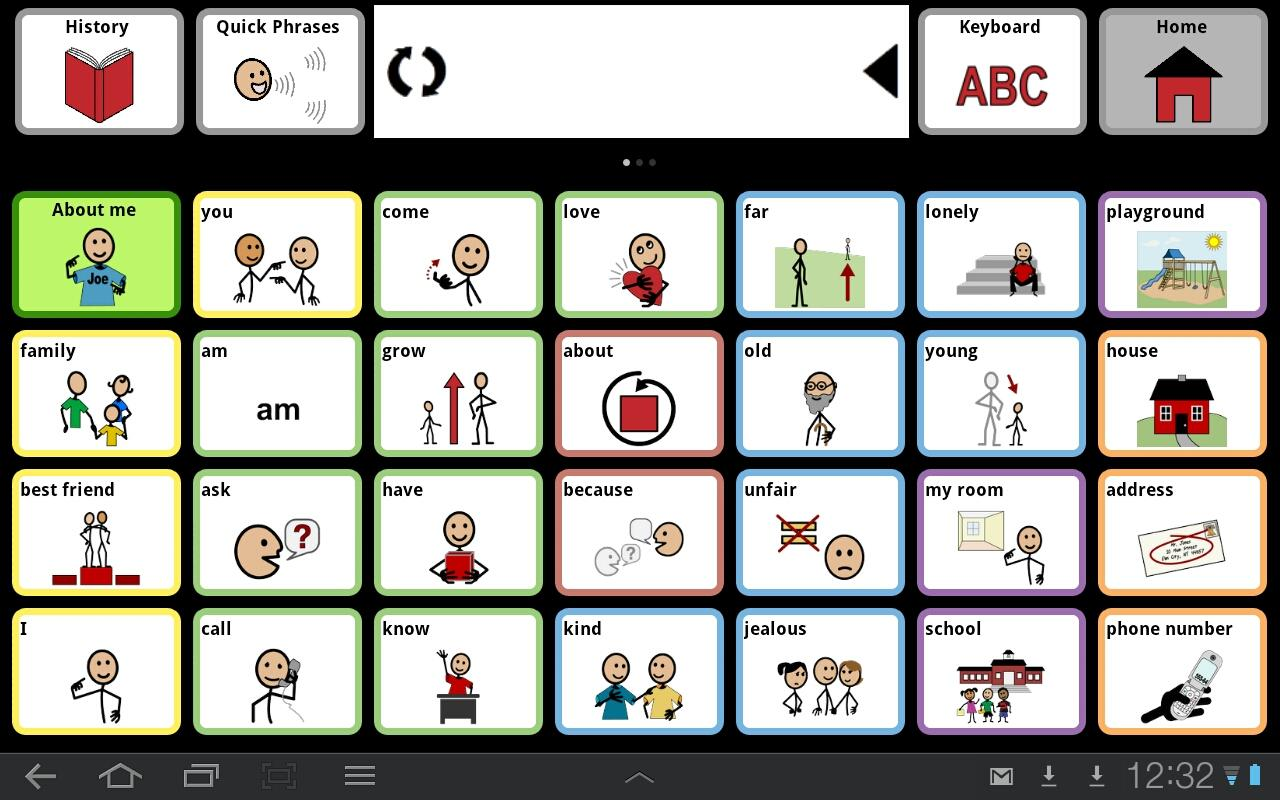
\includegraphics[width=150mm]{SonoFlex2}
\caption{Skjermdump av ASK programvaren Sono Flex}
\label{fig:SonoFlex}
\end{figure}


\section{Målsetninger}

Utgangspunktet til oppgaven var å se på måter som kunne forbedre designet til Sono flex. Det ble derimot tidlig i startfasen avklart at Tobii ikke ønsket at utviklingen skulle skje på deres eksisterende kode. Grunnen er at den eksisterende teknologien som programvaren er bygget på begynner å bli utdatert. Den eksisterende teknologien og koden er i god stand, men ikke optimal for de ønskede forbedringene. 

Målet med oppgaven har derfor blitt todelt. Det vil si at i tillegg til å bygge ut funksjoner og teste disse på den eksisterende programvaren, vil også programvaren som disse skal fungere på utvikles. Første delmål av oppgaven vil derfor være å utvikle programvaren. Andre delmål vil være å teste ulike design og funksjoner.

\subsection{Første delmål: Prototype}

På grunn av begrenset med tid og ressurser ville det ikke være mulig  utvikle en fullverdig versjon av den eksisterende løsningen Sono Flex. Planen ble derfor å bygge en high-fidelity prototype hvor kun hovedfunksjonaliteten var prioritert. High-fidelity vil si at prototypen er svært likt det endelige produktet, med mye detaljer og funksjonalitet \cite{Usabi1:online}. En high-fidelity prototype er såpass lik sluttproduktet at brukervennlighetstesting av den, vil gi sterke konklusjoner om hvordan atferd i det endelig produktet vil være. Med "reverse engineering" menes det at prototypen vil bli bygget ved å se og analyse funksjonaliteten til Sono Flex og ikke ved å se på koden. Det vil si at funksjonaliteten og det meste av utseende ville være det samme, men at implementasjonen og teknologien ville bli annerledes.


Når en først skulle starte et nytt prosjekt ble det bestemt at det burde fokuseres på kodekvalitet. God kode hadde uansett vært i fokus, men i denne sammenheng menes det litt utover det. Istedenfor å kun ha hovedfokus på å implementere funksjonalitet, så bør den være implementert slik at den følger standarder og mønster. Tankegangen var at ved å gjøre dette ville det være mulig å bruke prototypen i fremtidige prosjekter. Det økte også muligheten for at prototypen kunne videreutvikles til et ferdig prosjekt. 

Minstekravet til prototypen var at den skulle gi brukeren mulighet til å sette sammen enkle setninger å spille disse av som lyd. De ulike ordene skulle bli delt inn i tilhørende kategori. 


\subsection{Andre delmål: Forbedret brukervennlighet}
\label{sec:ResearchQuestion}

For å utforske mulige løsninger som kan øke brukervennligheten til Sono Flex vil en rekke funksjoner og design implementeres og testes. Først skal vi se på hvordan animasjon og lyd kan hjelpe en bruker med å finne ønsket symbol raskere. Deretter ønsket vi å finne en måte å gjøre det mulig for en bruker å endre innstillinger kun ved å bruke øyene. Vi velger å kalle dette øyestyrt brukertilpasning. Til slutt vil vi utforske veier en kan organisere og kategorisere ord på, for best å legge tilrette for et barn. Listen nedenfor gir en  beskrivelse av det vi ønsker å utforske.

\begin{enumerate} 
\label{lst:features}
\item Animasjon. Undersøk mulige fordeler forskjellige visualiseringseffekter kan ha på navigering innen og mellom sider og kategorier.
\item Lydeffekter. Undersøk mulige fordeler forskjellige lydeffekter kan ha på navigering innen og mellom sider og kategorier.
\item Optimal organisering og kategorisering. Hvordan skal knapper bli organisert og kategorisert for best å legge til rette for og forenkle navigasjon
\item Brukertilpasning. Mennesker har forskjellige preferanser, derfor er det i de fleste programvarer mulig for en bruker å tilpasse etter ønske. I dette tilfelle ønsker vi å gjøre dette mulig gjennom øyestyring. Spesifikk vil vi se på mulighetene for tilpasning av symbolstørrelse, animasjonsfart, farger og generelle innstillinger. 
\end{enumerate}

Forskningen vil bli gjort ved å implementere et program basert på en eksisterende løsning. De ulike forbedringene beskrevet i listen vil bli integrert.

\section{Testing}

Som nevnt i seksjon \ref{sec:ResearchQuestion}, er oppgaven å forbedre en type kommunikasjonsprogramvare for mennesker med komplekse kommunikasjonsvansker. For å undersøke virkningene til de forskjellige funksjonene, vil de prøves ut på en testgruppe.

For å få til dette, vil et utvalg av deltakerne prøve systemet uten tilleggsfunksjonene, mens de gjenværende vil forsøke med funksjonene. Mens deltagerne kjører programmet vil deres interaksjon med programmet bli lagret i en logg. Informasjonen fra undersøkelsen vil vise hvordan brukeren navigerte og hvor lang tid de brukte. Dette kan igjen brukes til å verifisere om en funksjon er en forbedring eller ikke.

\subsection{Målgruppe}

I kapittel \ref{sec:motivasjon} nevnes det at det er flere unge mennesker som helt eller delvis mangler tale. Som en konsekvens av dette har de behov for andre uttrykksformer for å kommunisere. Alternative uttrykksformer kan være håndtegn, symboler eller fotografier. Personer bruker ASK enten fordi det er et behov for å erstatte talen eller for å supplere utydelig eller svak tale.

International Society for Augmentative and Alternative Communication (\gls{isaac}) \cite{HvaErASK} definerer ASK som alt som hjelper en person til å kommunisere effektivt når tradisjonelle måter å kommunisere på ikke strekker til.

Målgruppen er personer som har behov for ASK systemer. Mer spesifikk vil programvaren være rettet mot: (A) Mennesker som ikke har mulighet for tale- og kroppsspråk,  (B) personer som ikke håndterer skriftspråk og (C) de som er nybegynnere på symbolbasert kommunikasjon. Dette gjelder hovedsakelig barn i alderen 2 til 5 år, men også eldre med mentale begrensninger. Videre i dette prosjektet vil personer som møter disse kriteriene bli omtalt som barn med komplekse kommunikasjonsbehov. 


\section{Oppsummering}

Tobii Dynavox vil utforske potensielle forbedringer i deres programvare. Problemet er at den eksisterende teknologien ikke er tilstrekkelig. Dette gjør at før vi kan utvikle og teste mulige forbedringer, må en prototype utvikles. Målet for oppgaven blir derfor først å utvikle prototype, deretter implementere mulige forbedringer.